\chapter{ポンプ圧力の差による周波数応答の変化}
油圧システムにおいて供給される圧力は重要な要素であり,圧力変化がシステムに与える影響を調べることは重要である.
そこで本章では,供給される圧力が変化した際のシステムの周波数応答について述べる.

手法として,ポンプの吐出圧力を\SI{7}{MPa},\SI{3.5}{MPa},\SI{1.0}{MPa}と変化させ,それぞれにおいて\ref{sec:SystemIdentification}章と同様に周波数応答を調べた.
なお,実験機で使用するサーボバルブの最低動作圧力が\SI{1.0}{MPa}である.
%先日のフルードパワーシステム学会においては$G_2$を用いて出力を推定する手法を提案した.
%この$G_2$に対してポンプからの吐出圧力$p_\mathrm{p}$が与える影響は大きく,モデル化誤差の要因になっていると予想される.
%そこで,ポンプ圧力$P\mathrm{p}$を\SI{7.0}{MPa},\SI{3.5}{MPa},\SI{1.0}{MPa}としたときの各周波数応答を調べる.
バルブへの指令電圧入力から実測出力までの周波数応答を\figname\ref{fig:1018_manubode_in2fmea}に,バルブ入力から推力までの周波数応答を\figname\ref{fig:1018_manubode_in2fthr}に,推力から出力までの周波数応答を\figname\ref{fig:1018_manubode_fthr2fmsr}にそれぞれ示す.
\figname\ref{fig:1018_manubode_fthr2fmsr}においてポンプ圧力\SI{7}{MPa}と\SI{3.5}{MPa}で周波数応答はほぼ一致していることから,ポンプに多少の圧力変動が存在しても,推力から出力までの伝達関数は変化しないとみなして良いといえる.


\begin{figure}[b]
	\centering
		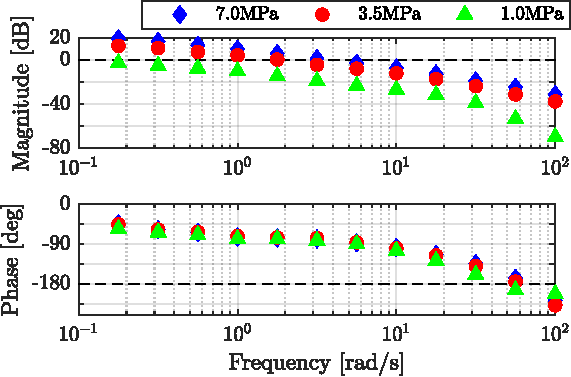
\includegraphics[keepaspectratio, scale = .9]{contents/Appendix_DiffPressure/figure/crop-1018_manubode_in2fmea.pdf}
		\caption{input to $\fmsr$}
		\label{fig:1018_manubode_in2fmea}
\end{figure}
\begin{figure}[t]
	\centering
		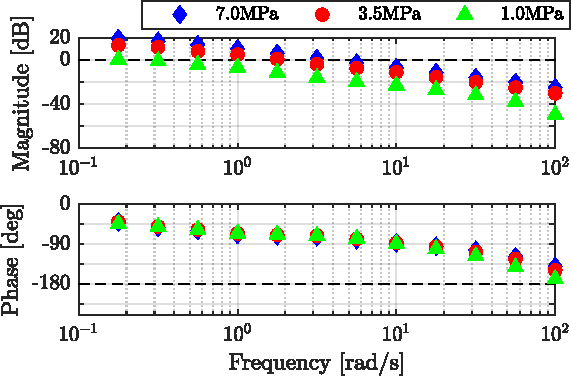
\includegraphics[keepaspectratio, scale = .9]{contents/Appendix_DiffPressure/figure/crop-1018_manubode_in2fthr.pdf}
		\caption{input to $\fthr$}
		\label{fig:1018_manubode_in2fthr}
\end{figure}
\begin{figure}[t]
	\centering
		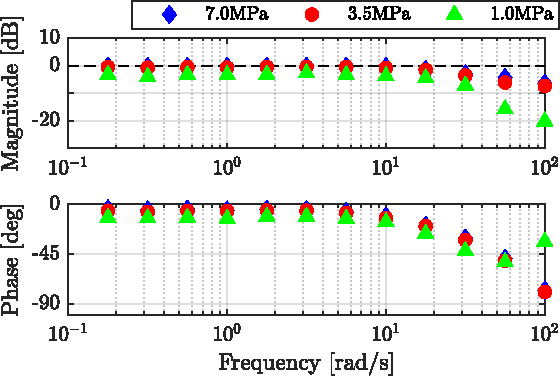
\includegraphics[keepaspectratio, scale = .9]{contents/Appendix_DiffPressure/figure/crop-1018_manubode_ftr2fmea.pdf}
		\caption{$\fthr$ to $\fmsr$}
		\label{fig:1018_manubode_fthr2fmsr}
\end{figure}